% Seção 7: dilatância e resposta depois da ruptura
The dilatancy changes the critical intensity and, above all, what the coupled transient does after it
(Figs.~\ref{fig:fstempo} and \ref{fig:decomp}). Without dilatancy ($\psi=0$) the coupled transient of model (i) loses
equilibrium for $I_r\ge26\mmh$, between 21.5~h (26~mm/h) and 11.75~h (180~mm/h); with 22~mm/h it does not. With
$\psi=\phi'/2$ or $\psi=\phi'$ the minimum FS stays between 1.000 and 1.008 from 36 to 180~mm/h and the transient never
loses equilibrium: the slope is at limit equilibrium, within the resolution of the FS, without collapse of the
transient. Below the critical intensity the flow rule hardly matters: with 18~mm/h the minimum FS is 1.316 with
$\psi=0$ and 1.319 with $\psi=\phi'/2$ and $\phi'$. With $\delta=0.01$ the critical intensity is 26~mm/h with $\psi=0$
and 31~mm/h with $\psi=\phi'$ (20\% higher); with $\psi=0$ the failure occurs 5.4--6.3~h earlier in the rainfalls of 54
and 90~mm/h (Table~\ref{tab:decomp}). With $\psi=\phi'/2$ only 18 and 36~mm/h were computed below 54~mm/h, so its
critical intensity is only known to lie between 18 and 36~mm/h.

\begin{figure}[htbp]
\centering
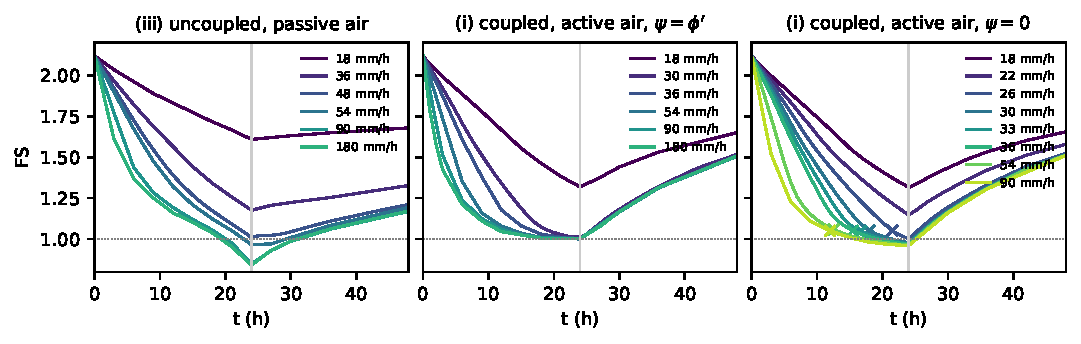
\includegraphics[width=\textwidth]{fs_tempo.pdf}
\caption{FS during and after 24-h rainfalls of several intensities, soil $f_{50}$, $\alpha=45^\circ$: model (iii)
and model (i) with $\psi=\phi'$ and $\psi=0$ ($\times$: loss of equilibrium of the coupled transient; afterwards the
transient continues with the strength increased, only to follow the pressures).}\label{fig:fstempo}
\end{figure}

With $\psi=0$ the loss of equilibrium occurs when the FS of the strength reduction, computed with $\psi=\phi'$, is
still 1.047--1.059. Either the associated strength reduction overestimates by about 5\% the FS of a soil without
dilatancy, or part of the loss of equilibrium is numerical; the time step does not explain it: with a time step of
0.125~h instead of 0.25~h during the rainfall, the transient with 36~mm/h loses equilibrium after 15.6~h instead of
15.5~h. For $\psi=0$ the time of failure is therefore $t_f$, and $22<\Ic\le26\mmh$ by the loss of equilibrium. The
FS values below one after $t_f$ use the pressures of a transient continued with the strength increased and only show
that the equilibrium was exceeded.

The flow rule matters as much with passive air. In model (ii) the transient without dilatancy loses equilibrium
after 22.3~h with 54~mm/h, and its critical intensity is 53~mm/h; with $\psi=\phi'$ the minimum FS is 1.033, 1.014,
1.010 and 1.009 with 54, 66, 78 and 90~mm/h, and the transient never loses equilibrium. In both coupled models,
the transients with an associated flow rule do not collapse in the range computed, and those without dilatancy do. The
mechanism (for instance the suction generated by the plastic dilation of the shear zone) was not isolated here.
